\def\pgfsysdriver{pgfsys-dvisvgm.def}
% flashcards-title: Two candidate boundaries around a plant system
% flashcards-desc: Two panels contain the same plant, soil, and air components. Candidate A encloses only the plant; Candidate B encloses the plant, soil, and nearby air. Arrows show possible effects.
\documentclass[tikz,border=6pt]{standalone}
\usetikzlibrary{arrows.meta,calc,fit,positioning,shapes.geometric}

\definecolor{fcink}{HTML}{17212B}
\definecolor{fcblue}{HTML}{1D5D8C}
\definecolor{fcgreen}{HTML}{2D6A4F}
\definecolor{fcorange}{HTML}{A44A1F}
\definecolor{fcpale}{HTML}{F4F7F9}
\definecolor{fcsoil}{HTML}{8B5E3C}

\tikzset{
  fc text/.style={font=\sffamily, text=fcink},
  fc panel/.style={draw=fcink, line width=0.9pt, rounded corners=5pt, fill=fcpale},
  fc node/.style={draw=fcink, line width=0.9pt, rounded corners=4pt, fill=white,
    minimum width=24mm, minimum height=10mm, align=center, font=\sffamily},
  fc arrow/.style={-{Stealth[length=3.2mm,width=2.4mm]}, line width=1.2pt,
    draw=fcblue, line cap=butt},
  fc boundary/.style={draw=fcorange, line width=1.4pt, dash pattern=on 5pt off 3pt,
    rounded corners=7pt},
  fc label/.style={font=\sffamily\bfseries, text=fcink},
  fc note/.style={font=\sffamily\small, text=fcink, align=center}
}

\begin{document}
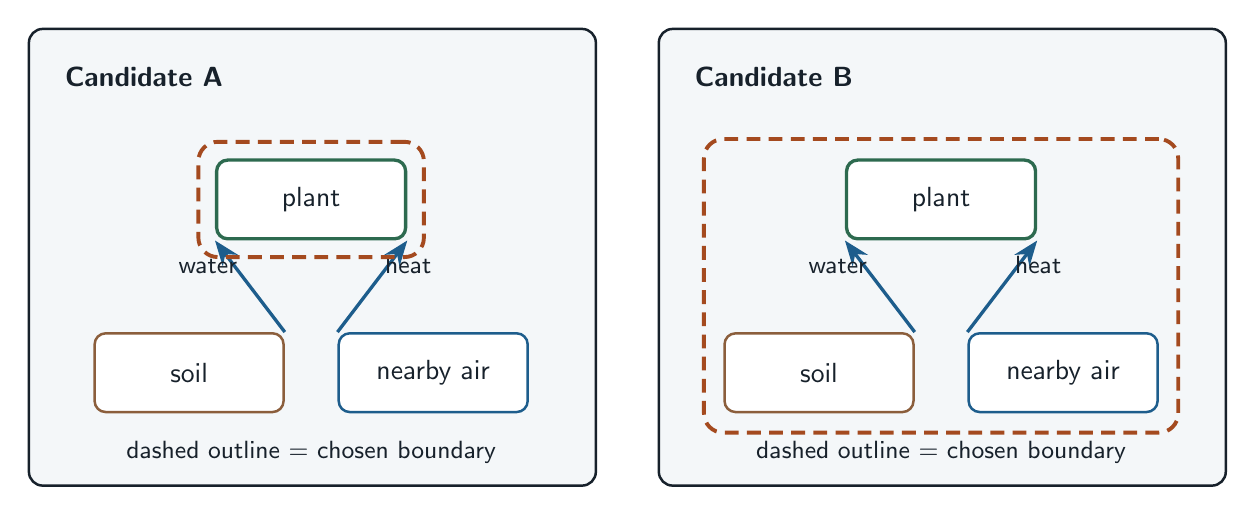
\begin{tikzpicture}[fc text, x=1cm, y=1cm]
  \node[fc panel, minimum width=72mm, minimum height=58mm, anchor=south west] (pa) at (0,0) {};
  \node[fc panel, minimum width=72mm, minimum height=58mm, anchor=south west] (pb) at (8.0,0) {};

  \node[fc label, anchor=north west] at (0.35,5.45) {Candidate A};
  \node[fc label, anchor=north west] at (8.35,5.45) {Candidate B};

  \node[fc node, draw=fcgreen, line width=1.2pt] (plantA) at (3.6,3.65) {plant};
  \node[fc node, draw=fcsoil] (soilA) at (2.05,1.45) {soil};
  \node[fc node, draw=fcblue] (airA) at (5.15,1.45) {nearby air};
  \draw[fc arrow] (soilA.north east) -- node[fc note, above left=1pt] {water} (plantA.south west);
  \draw[fc arrow] (airA.north west) -- node[fc note, above right=1pt] {heat} (plantA.south east);

  \node[fc node, draw=fcgreen, line width=1.2pt] (plantB) at (11.6,3.65) {plant};
  \node[fc node, draw=fcsoil] (soilB) at (10.05,1.45) {soil};
  \node[fc node, draw=fcblue] (airB) at (13.15,1.45) {nearby air};
  \draw[fc arrow] (soilB.north east) -- node[fc note, above left=1pt] {water} (plantB.south west);
  \draw[fc arrow] (airB.north west) -- node[fc note, above right=1pt] {heat} (plantB.south east);

  \node[fc boundary, fit=(plantA), inner sep=6pt] {};
  \node[fc boundary, fit=(plantB)(soilB)(airB), inner sep=7pt] {};

  \node[fc note, anchor=south] at (3.6,0.18) {dashed outline = chosen boundary};
  \node[fc note, anchor=south] at (11.6,0.18) {dashed outline = chosen boundary};
\end{tikzpicture}
\end{document}
